\documentclass[a4paper,12pt]{article}
\usepackage[T2A]{fontenc}
\usepackage[utf8]{inputenc}
\usepackage[english,russian]{babel}
\usepackage{listings}

\usepackage{amsmath}
\usepackage{MnSymbol}
\usepackage{wasysym}
\usepackage{indentfirst}
\usepackage[unicode, pdftex]{hyperref}

\usepackage{pgfplots}
\pgfplotsset{compat=1.9}

\usepackage{geometry}
\geometry{left=2cm}
\geometry{right=1.5cm}
\geometry{top=1cm}
\geometry{bottom=2cm}

\usepackage{graphicx}
\graphicspath{{img/}}
\DeclareGraphicsExtensions{.pdf,.png,.jpg}

\newcommand{\anonsection}[1]{\section*{#1}\addcontentsline{toc}{section}{#1}}

% переименовываем  список литературы в "список используемой литературы"
\addto\captionsrussian{\def\refname{Список используемой литературы}}

\lstset{
    language=C++,
    numbers=left,
    frame=single,
    texcl=true,
    basicstyle=\ttfamily
}

\begin{document}

\begin{titlepage}

    \begin{center}
        \large
        Государственное образовательное учреждение высшего профессионального образования\\
        “Московский государственный технический университет имени Н.Э.Баумана”
        \vspace{3cm}

        \textsc{Дисциплина: Анализ алгоритмов}
        \vspace{0.5cm}

        \textsc{Лабораторная работа №1}
        \vspace{3cm}

        {\LARGE РЕДАКЦИОННОЕ РАССТОЯНИЕ}
        \vspace{3cm}

        Студент группы ИУ7-53,\\
        Степанов Александр Олегович
        \vfill
    \end{center}

    \begin{flushright}
        \begin{tabular}{l}
            Преподаватели:\\
            Строганов Юрий Владимирович\\
            Волкова Лилия Леонидовна
        \end{tabular}
    \end{flushright}

    \begin{center}

        2019 г.

    \end{center}

\end{titlepage}

\tableofcontents

\newpage
\anonsection{Введение}

В настоящее время большую популярность имеют поисковики, в которых для удобства
пользователя необходимо исправлять ошибки. Подобные ошибки в словах могут возникнуть
также в базах данных, при распозновании отсканированного текста или речи, или
при обычном вводе текста. Подобная проблема решается с помощью редакционного
расстояния. \cite{habr}
Самыми популярными алгоритмами поиска редакционного расстояния являются
расстояние Левенштейна и Демарау-Левенштейна, которые активно применяются:

\begin{itemize}
    \item для исправления ошибок в слове (в поисковых системах, базах
        данных, при вводе текста, при автоматическом распознавании
        отсканированного текста или речи) \cite{habr};

    \item для сравнения текстовых файлов утилитой diff и ей подобными;

    \item в биоинформатике для сравнения генов, хромосом и белков \cite{bio}.
\end{itemize}

В данной лабораторной работе ставятся следующие задачи:

\begin{enumerate}
    \item Изучение алгоритмов Левенштейна и Дамерау-Левенштейна нахождения
        расстояния между строками
    \item Получение практических навыков реализации указанных алгоритмов:
        двух алгоритмов в матричной версии и оного из алгоритмов в рекурсивной
        версии
    \item Сравнительный анализ линейной и рекурсивной реализации выбранного
        алгоритма определения расстояния между строками по затрачиваемым
        ресурсам (времени и памяти)
    \item Экспериментальное подтверждение различий во временой эффективности
        рекурсивной и нерекурсивной реализации выбранного алгоритма
        определения расстояния межлу строками при помощи разработанного
        программного обеспечения на материале замеров процессорного времен
        выполнения реализации на варьирующихся длинах строк
\end{enumerate}

\newpage
\section{Аналитическая часть}

Редакционное расстояние активно применяется в программировании и биоиформатике.
Самые популярные алгоритмы поиска редакционного расстояния это алгоритм
Левенштейна и Дамерау-Левенштейна \cite{habr}.

\subsection{Описание задачи}

\textbf{Редакционное расстояние (расстояние Левенштейна)}
между двух строк - это
минимальное количество операций вставки одного символа, удаления одного
символа или замены одного символа на другой необходимых для превращения
одной строки в другую. \cite{itmo}

Для двух строк $S_1$ и $S_2$ с длинами $n$ и $m$ соотвественно можно
построить матрицу $D(n+1, m+1)$, в которой каждый элемент вычисляется по формуле (1)
\cite{itmo}

\begin{equation}
D(i,j) =
\begin{cases}
    0, \text{ если } i = 0, j = 0 \\
    i, \text{ если } j = 0 \\
    j, \text{ если } i = 0 \\
    \min
    \left(
        \begin{matrix}
            D(i, j - 1) + 1 \\
            D(i - 1, j) + 1 \\
            D(i - 1, j - 1) +
            \begin{cases}
                0, \text{ если } S_1[i] \ne S_2[j] \\
                1, \text{ иначе}
            \end{cases}
        \end{matrix}
    \right)
    , \text{ иначе}
\end{cases}
\end{equation}

После нахождения каждого элемента матрицы, редакционное расстояние между
$S_1$ и $S_2$ будет в нижнем правом элементе матрицы.

\textbf{Расстояние Дамерау-Левенштейна} - это редакционное расстояние,
к которому добавляется еще одно действие - транспозиция (смена местами
двух соседних символов). Необходимо это потому, что около 80\% ошибок
при наборе текста человеком является транспозиция, как показал Дамерау. \cite{bmstu}

По аналогии с расстоянием Левенштейна, здесь тоже используется матрица
$D(n+1, m+1)$ для строк $S_1$ и $S_2$ с длинами $n$ и $m$ уже по формуле (2)
\cite{bmstu}

\begin{equation}
D(i,j) =
\begin{cases}
    0, \text{ если } i = 0, j = 0 \\
    i, \text{ если } j = 0 \\
    j, \text{ если } i = 0 \\

    \min
    \left(
        \begin{matrix}
            D(i, j - 1) + 1 \\
            D(i - 1, j) + 1 \\
            D(i - 1, j - 1) +
            \begin{cases}
                1, \text{ если } S_1[i] \ne S_2[j] \\
                0, \text{ иначе}
            \end{cases} \\
            D(i - 2, j - 2) + 1
        \end{matrix}
    \right) \\
    , \text{ если } i > 1, j > 1, S_1[i] = S_2[j - 1], S_2[j] = S_1[i - 1] \\

    \min
    \left(
    \begin{matrix}
        D(i, j - 1) + 1 \\
        D(i - 1, j) + 1 \\
        D(i - 1, j - 1) +
        \begin{cases}
            1, \text{ если } S_1[i] \ne S_2[j] \\
            0, \text{ иначе}
        \end{cases}
    \end{matrix}
    \right)
    , \text{ иначе}
\end{cases}
\end{equation}

\subsection{Пути решения}

Впервые эту задачу поставил советский математик Владимир Левенштейн при
изучении последовательностей 0-1. \cite{binlev}

После него Фредерик Дамерау доказал, что пользователи совершают очень много
ошибок транспозиции при наборе текста, и доработал алогоритм Левенштейна.
Поэтому расстояние Дамерау-Левенштейна дает более лучшие результаты, чем
обычное редакционное расстояние.

\subsection{Выводы}

Редакционное расстояние широко применяется в областях программирования и
биоинформатики. Для алгоритмов Левенштейна и Дамерау-Левенштейна
используются операции вставки символа, удаления символа, замены символа и
транспозиции двух соседних символов. В данной работе будет проведено
исследование и сравнение этих алгоритмов.

\newpage
\section{Конструкторская часть}

В данной работе для нахождения расстояния Левенштейна используется матричный
алгоритм, а для Дамерау-Левенштейна матричный и рекурсивный. Далее будут
рассмотрены все эти алгоритмы.

\subsection{Функциональная модель}

\begin{center}
    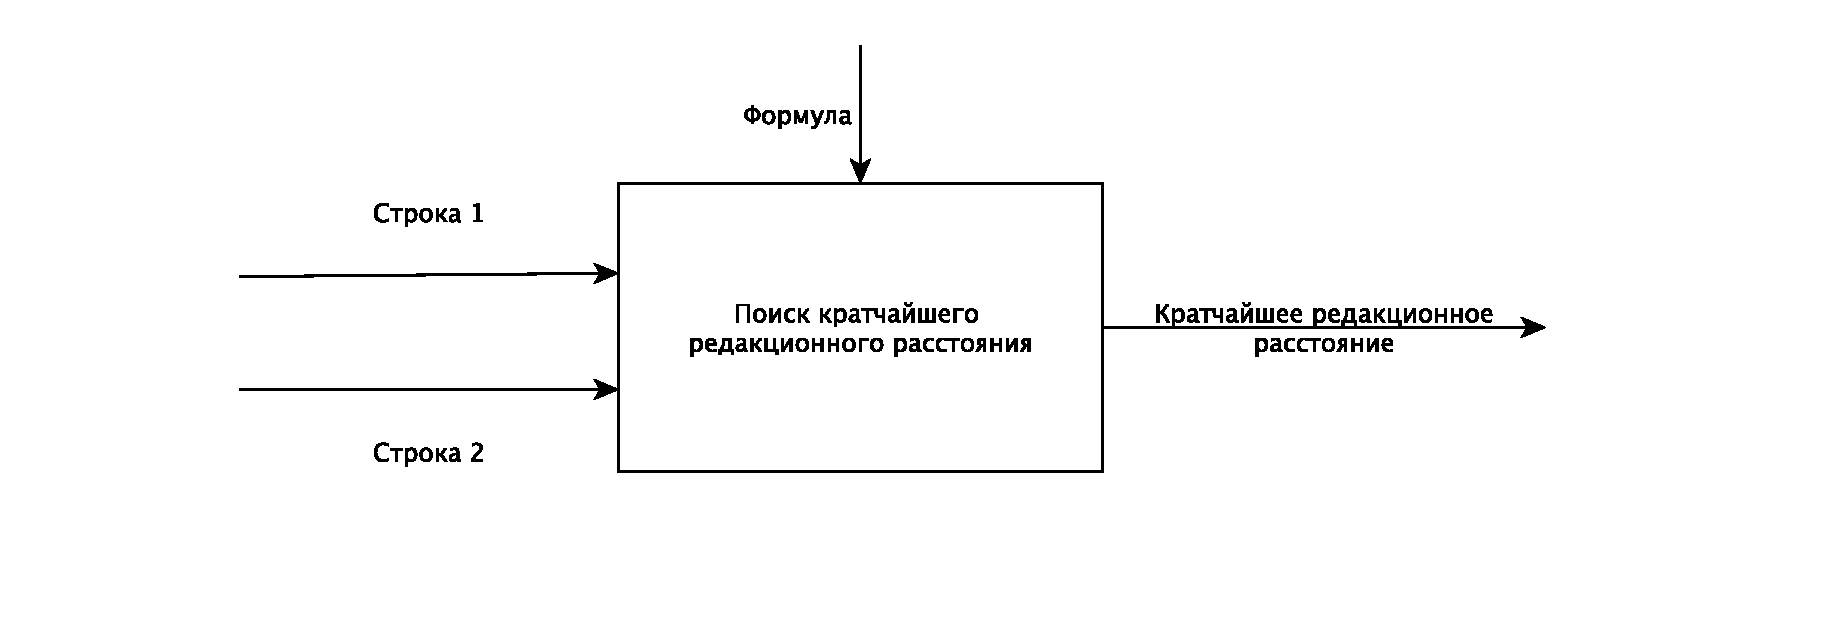
\includegraphics[scale=0.5]{IDEF0}

    Схема 1. IDEF0
\end{center}

\subsection{Схемы алгоритмов}

\subsubsection{Матричный алгоритм Левенштейна}

\begin{center}
    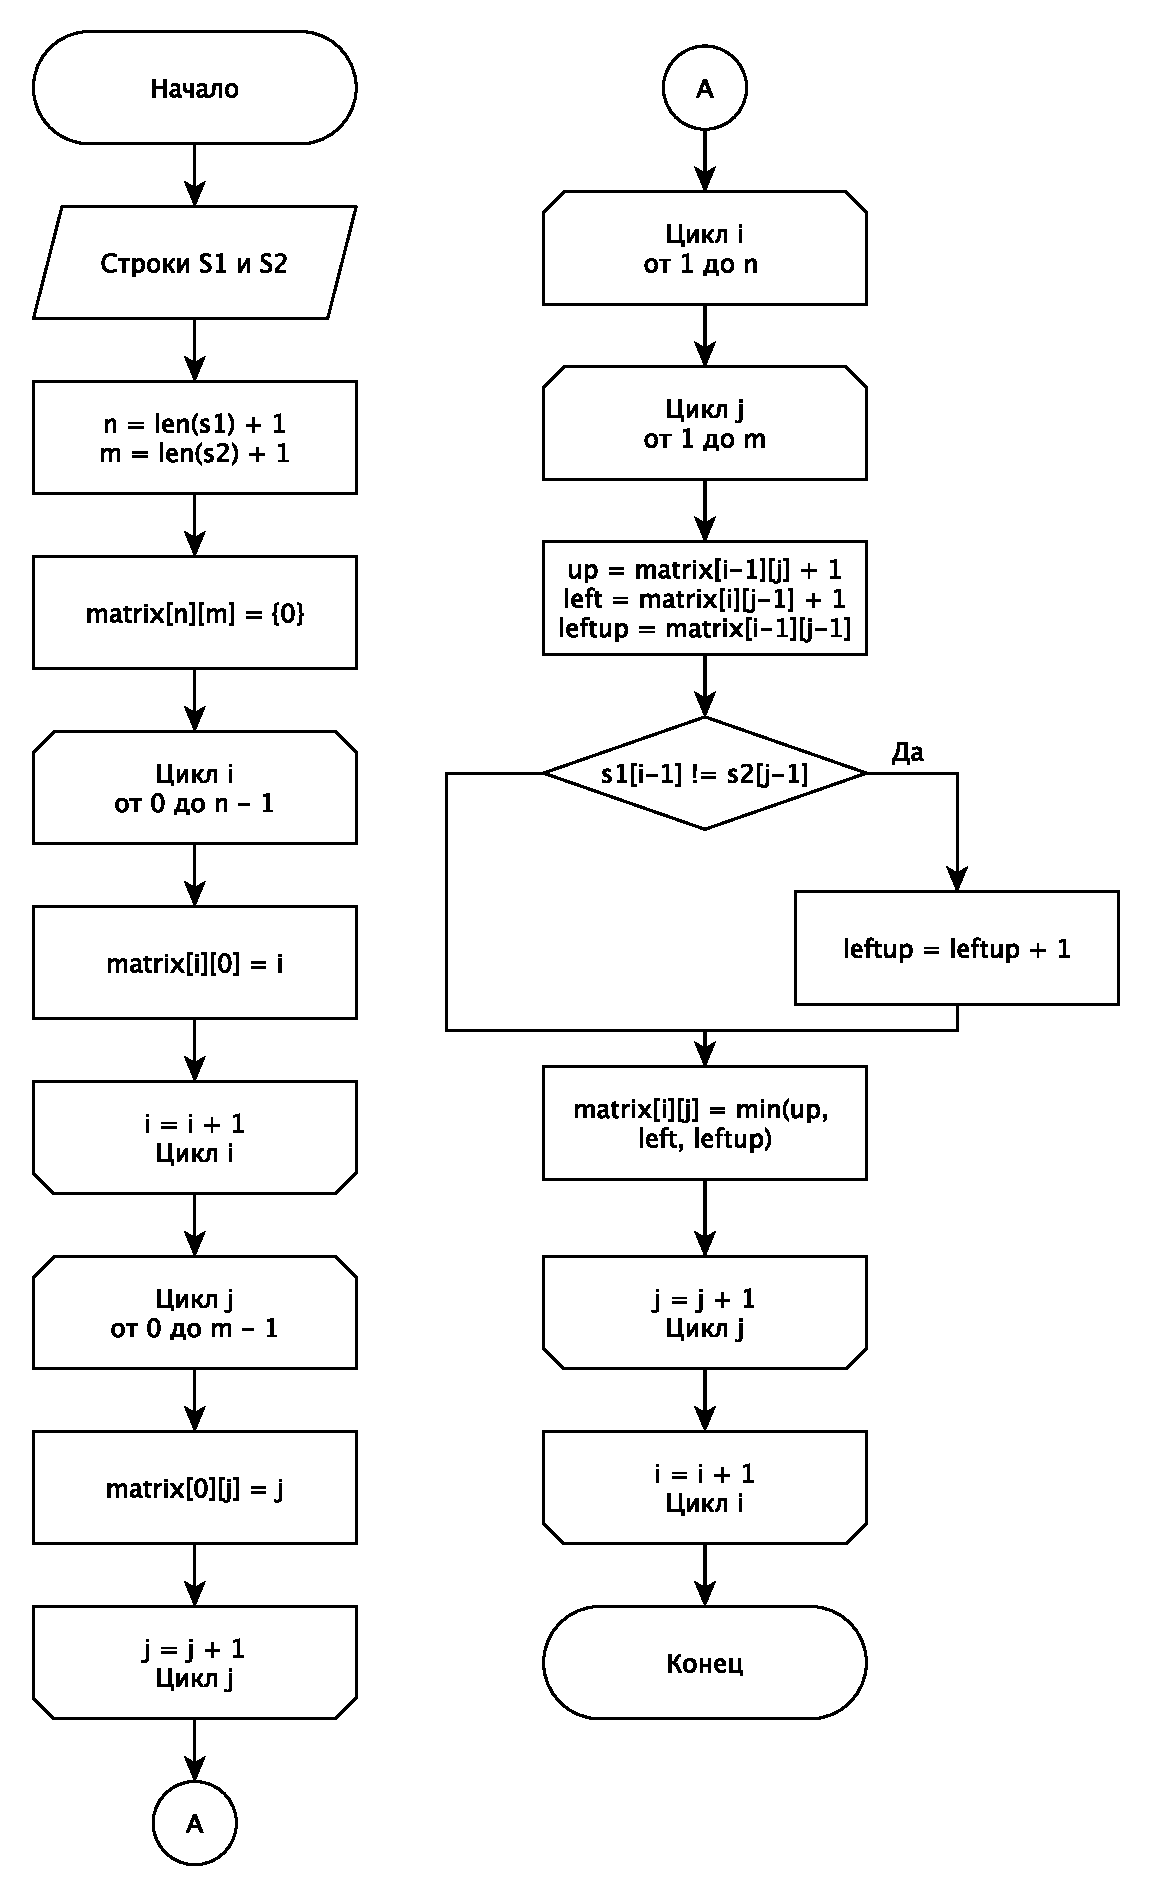
\includegraphics[scale=0.7]{Lmatrix}

    Схема 2. Матричный алгоритм Левенштейна
\end{center}

\subsubsection{Матричный алгоритм Дамерау-Левенштейна}

\begin{center}
    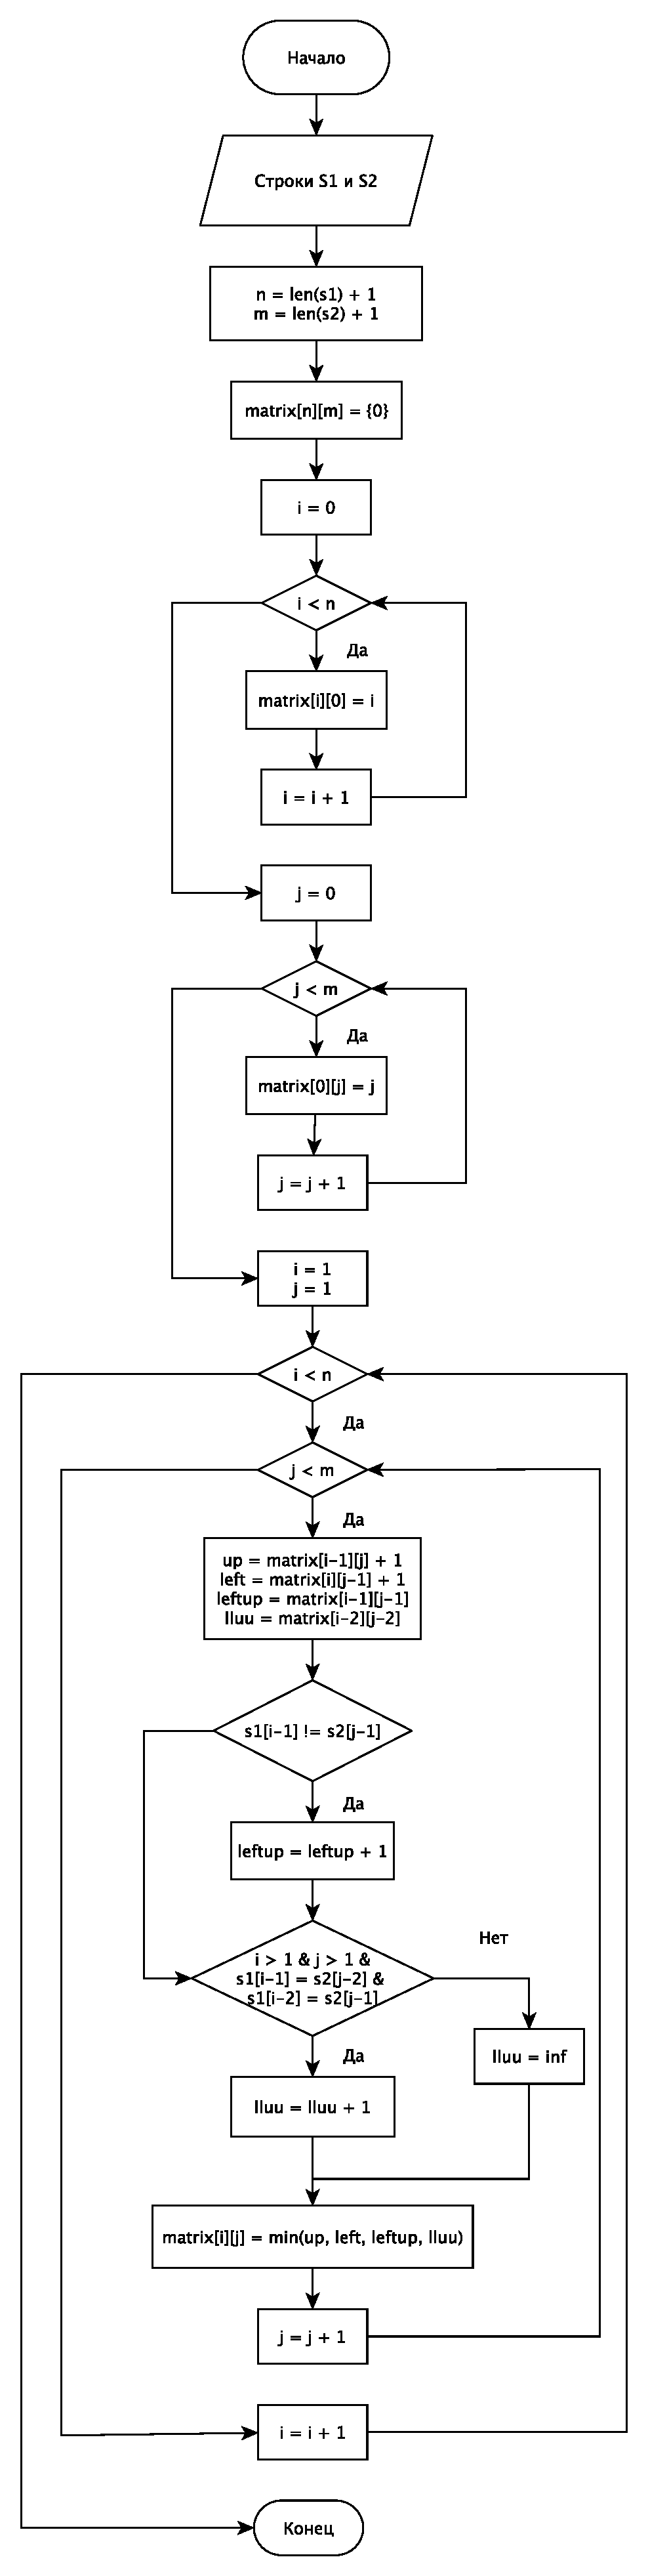
\includegraphics[scale=0.6]{DLmatrix}

    Схема 3. Матричный алгоритм Дамерау-Левенштейна
\end{center}

\subsubsection{Рекурсивный алгоритм Дамерау-Левенштейна}

\begin{center}
    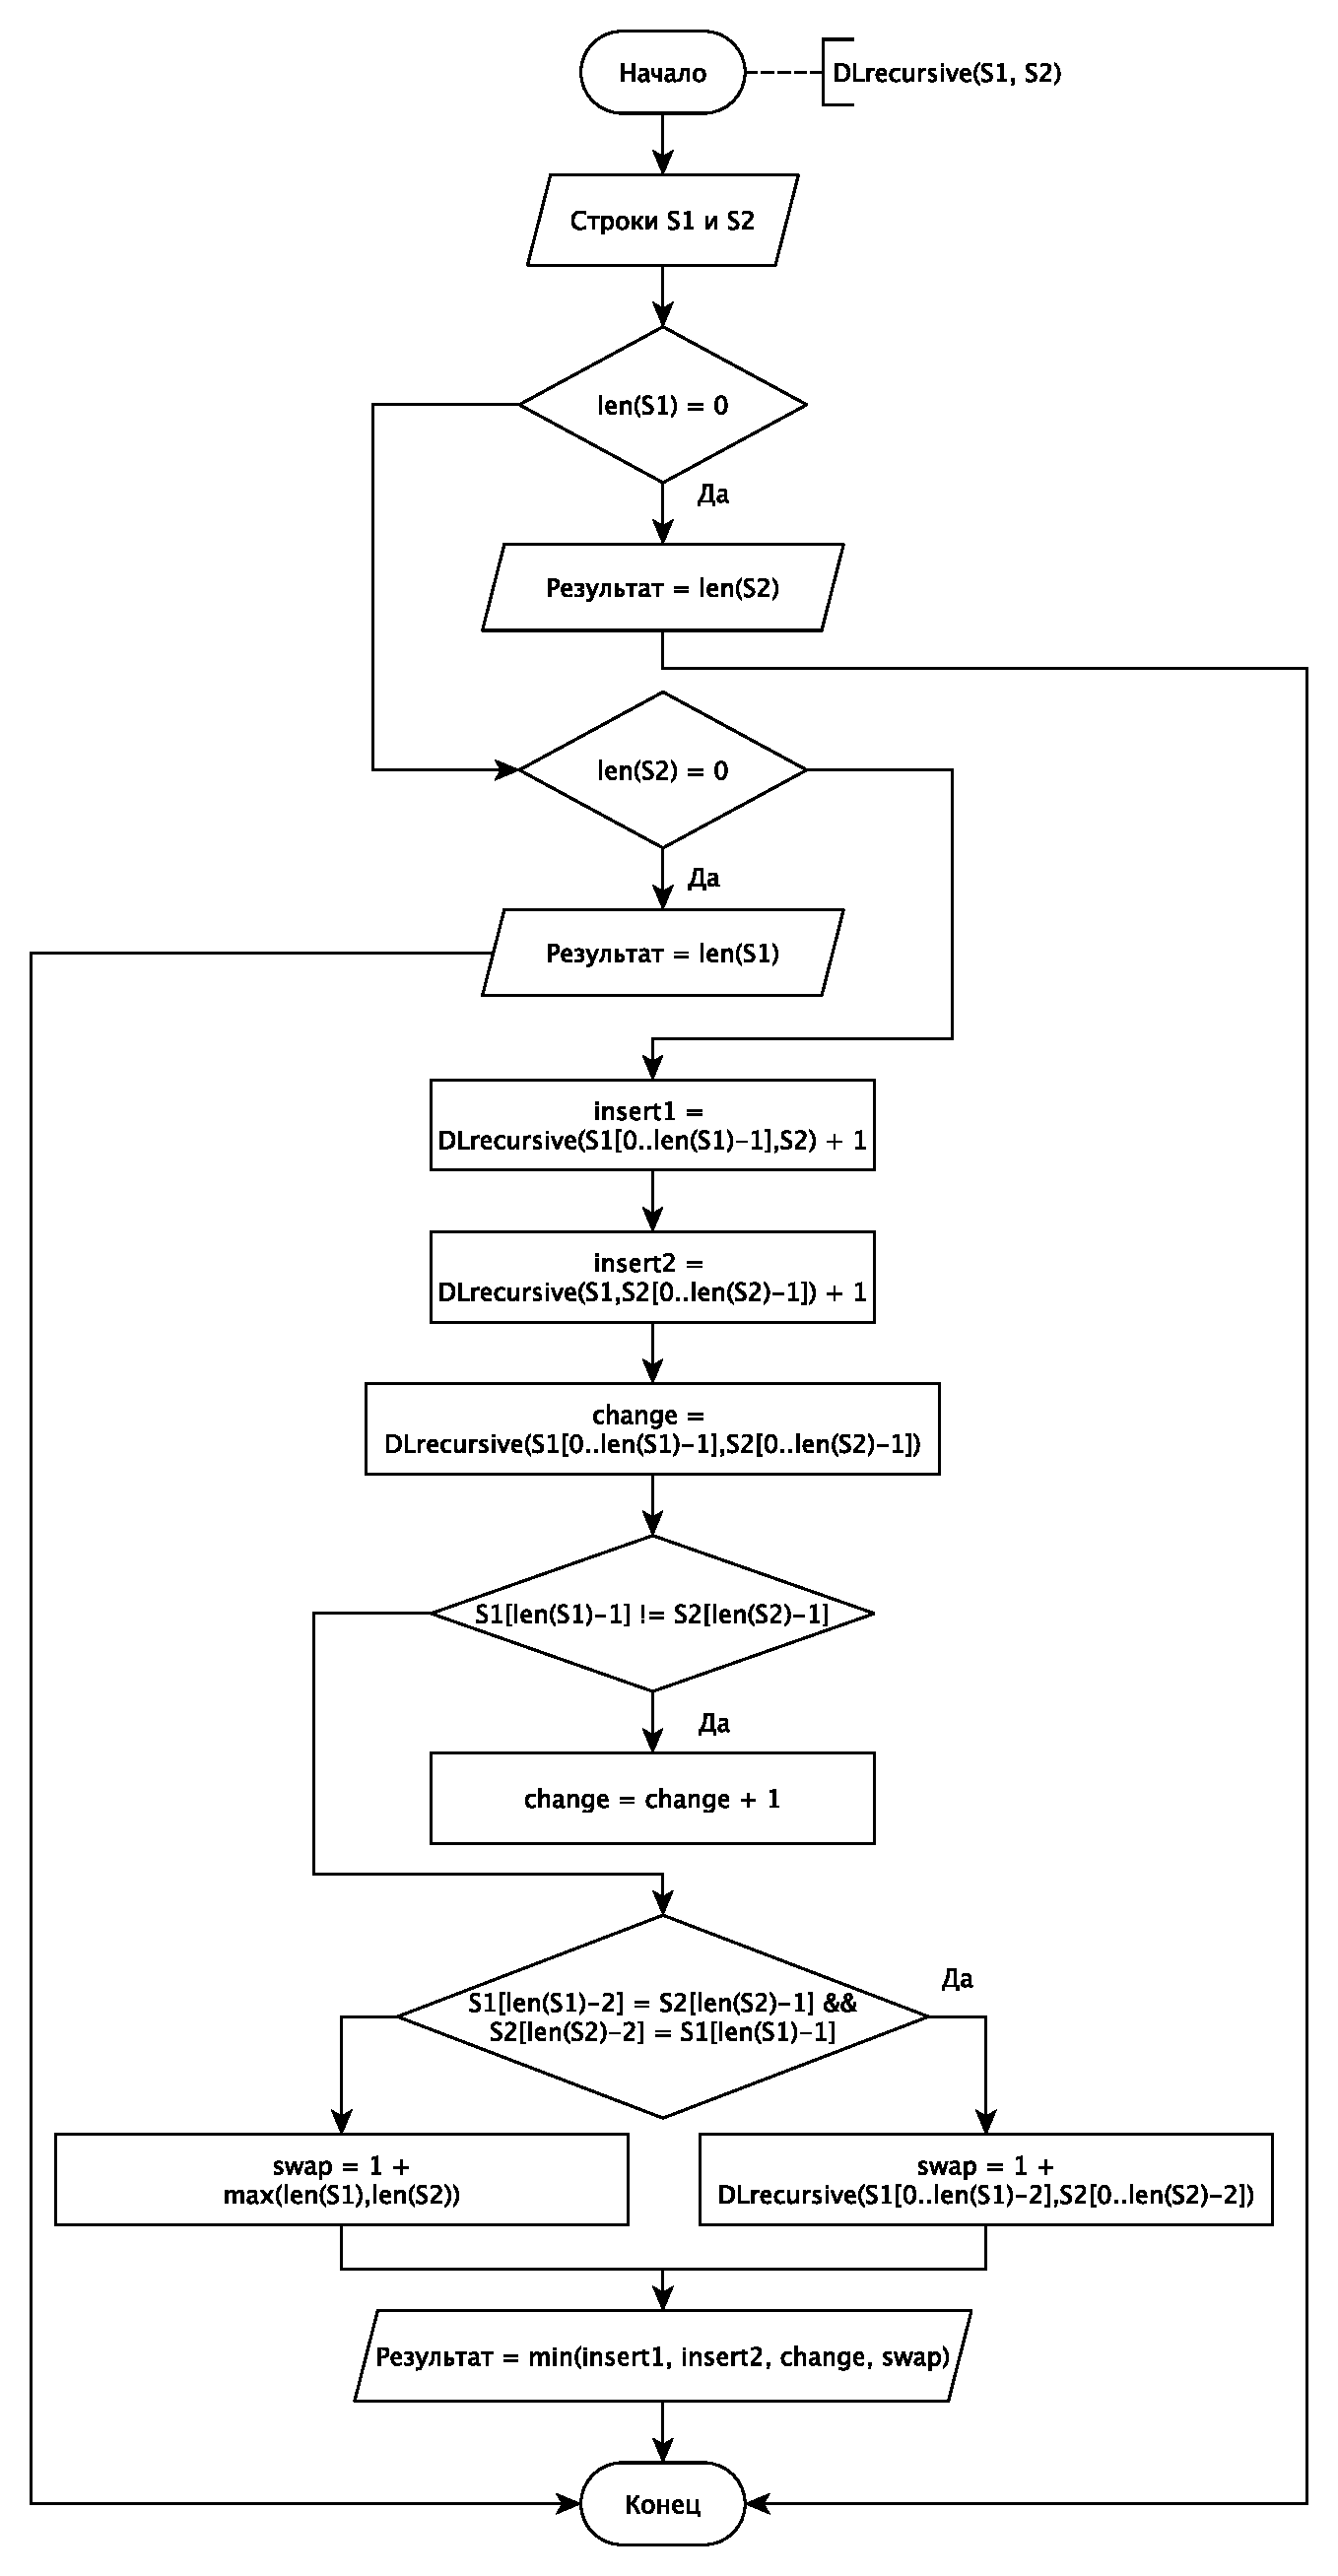
\includegraphics[scale=0.4]{DLrecursive}

    Схема 4. Рекурсивный алгоритм Дамерау-Левенштейна
\end{center}

\subsection{Выводы}

Рекурсивный алгоритм имеет сложность $\Omega (4^{max(n,m)})$, а матричные
$\Omega (n \cdot m)$. Таким образом очевидно, что рекурсивный алгоритм
сильно проигрывает матричным по времени. Проверим данное предположение
на реализованных алгоритмах.

\newpage
\section{Технологическая часть}

Необходимо определиться со средствами для разработки алгоритмов и подготовить
тесты.

\subsection{Требования к программному обеспечению}

Программное обеспечение должно обеспечивать замер процессорного времени
выполнения каждого алгоритма. Проводятся замеры для случайно генерируемых
строк размерности до 1000.

\subsection{Средства реализации}

В качестве языка программирования был выбран C++.
Данный язык имеет высокую скорость и богатую стандартную библиотеку,
содержащую необходимые контейнеры для данной работы. Программа, написанная на C++,
будет доступна на всех платформах.

\subsection{Листинг кода}

\begin{lstlisting}[caption=Расстояние Левенштейна матричный метод]
Matrix Lmatrix::find(std::string s1, std::string s2)
{
    Matrix matrix;
    for (int i = 0; i < s1.size() + 1; ++i) {
        matrix.push_back(std::vector< int >(s2.size() + 1));
    }

    for (int i = 0; i < matrix.size(); ++i) {
        matrix[i][0] = i;
    }

    for (int j = 0; j < matrix[0].size(); ++j) {
        matrix[0][j] = j;
    }

    for (int i = 1; i < matrix.size(); ++i) {
        for (int j = 1; j < matrix[0].size(); ++j) {
            int u = matrix[i - 1][j] + 1;
            int l = matrix[i][j - 1] + 1;
            int lu = matrix[i - 1][j - 1];
            if (s1[i - 1] != s2[j - 1]) lu++;

            matrix[i][j] = std::min(std::min(u, l), lu);
        }
    }

    return matrix;
}
\end{lstlisting}

\begin{lstlisting}[caption=Расстояние Дамерау-Левенштейна матричный метод]
Matrix DLmatrix::find(std::string s1, std::string s2)
{
    Matrix matrix;
    for (int i = 0; i < s1.size() + 1; ++i) {
        matrix.push_back(std::vector< int >(s2.size() + 1));
    }

    for (int i = 0; i < matrix.size(); ++i) {
        matrix[i][0] = i;
    }

    for (int j = 0; j < matrix[0].size(); ++j) {
        matrix[0][j] = j;
    }

    int inf = std::max(s1.size(), s2.size()) + 1;

    for (int i = 1; i < matrix.size(); ++i) {
        for (int j = 1; j < matrix[0].size(); ++j) {
            int u = matrix[i - 1][j] + 1;
            int l = matrix[i][j - 1] + 1;
            int lu = matrix[i - 1][j - 1];
            int lluu = inf;
            if (i > 1 && j > 1) lluu = matrix[i - 2][j - 2];

            if (s1[i - 1] != s2[j - 1]) lu++;
            if (lluu != -1 &&
                s1[i - 1] == s2[j - 2] &&
                s1[i - 2] == s2[j - 1])
                lluu++;
            else lluu = inf;

            matrix[i][j] = std::min(std::min(u, l),
                                    std::min(lu, lluu));
        }
    }

    return matrix;
}
\end{lstlisting}

\begin{lstlisting}[caption=Расстояние Дамерау-Левенштейна рекурсивный метод]
int DLrecursive::find(std::string s1, std::string s2)
{
    if (s1.size() == 0) return s2.size();
    if (s2.size() == 0) return s1.size();

    return std::min(
            std::min(
                find(s1.substr(0, s1.size() - 1), s2) + 1,
                find(s1, s2.substr(0, s2.size() - 1)) + 1
            ),
            std::min(
                find(s1.substr(0, s1.size() - 1),
                        s2.substr(0, s2.size() - 1)) +
                (s1[s1.size() - 1] == s2[s2.size() - 1] ? 0 : 1),

                (s1.size() > 1 &&
                s2.size() > 1 &&
                s1[s1.size() - 2] == s2[s2.size() - 1] &&
                s1[s1.size() - 1] == s2[s2.size() - 2] ?
                find(s1.substr(0, s1.size() - 2),
                        s2.substr(0, s2.size() - 2)) :
                    int(std::max(s1.size(), s2.size()))) + 1
            )
        );
}

\end{lstlisting}

\subsection{Тестирование}

Для тестирования программы были заготовлены следующие тесты

\hfill

\begin{center}
    \begin{tabular}{|c|c|c|}
        \hline
        $s_1$ & $s_2$ & Ожидаемый результат \\
        \hline
        word & word & 0 \\
        \hline
        word & another & 6 \\
        \hline
        ab & ba & 2 \\
        \hline
        qwerty & qwetry & 2 \\
        \hline
        abcdef & badcfe & 4 \\
        \hline
        werylongword & sh & 12 \\
        \hline
        sh & werylongword & 12 \\
        \hline
        wednesday & weekend & 5 \\
        \hline
        memory & mem & 3 \\
        \hline
        feature & erutaef & 6 \\
        \hline
    \end{tabular}

    Таблица 1. Тесты для алгоритма Левенштейна
\end{center}

\hfill

\begin{center}
    \begin{tabular}{|c|c|c|}
        \hline
        $s_1$ & $s_2$ & Ожидаемый результат \\
        \hline
        word & word & 0 \\
        \hline
        word & another & 6 \\
        \hline
        ab & ba & 1 \\
        \hline
        qwerty & qwetry & 1 \\
        \hline
        abcdef & badcfe & 3 \\
        \hline
        werylongword & sh & 12 \\
        \hline
        sh & werylongword & 12 \\
        \hline
        wednesday & weekend & 5 \\
        \hline
        memory & mem & 3 \\
        \hline
        feature & erutaef & 5 \\
        \hline
    \end{tabular}

    Таблица 2. Тесты для алгоритма Дамерау-Левенштейна
\end{center}

\subsection{Выводы}

Для сравнения были реализованы 3 алгоритма на выбранном языке
программирования C++. Чтобы проверить правильность работы алгоритмов
были подготовлены тесты.

\newpage
\section{Экспериментальная часть}

Проведем тестирование и сравним реализованные алгоритмы по времени.

\subsection{Примеры работ}

Ниже приведены примеры работ при корректных и некорректных данных


\includegraphics[scale=0.35]{zero_arg}


\includegraphics[scale=0.35]{one_arg}

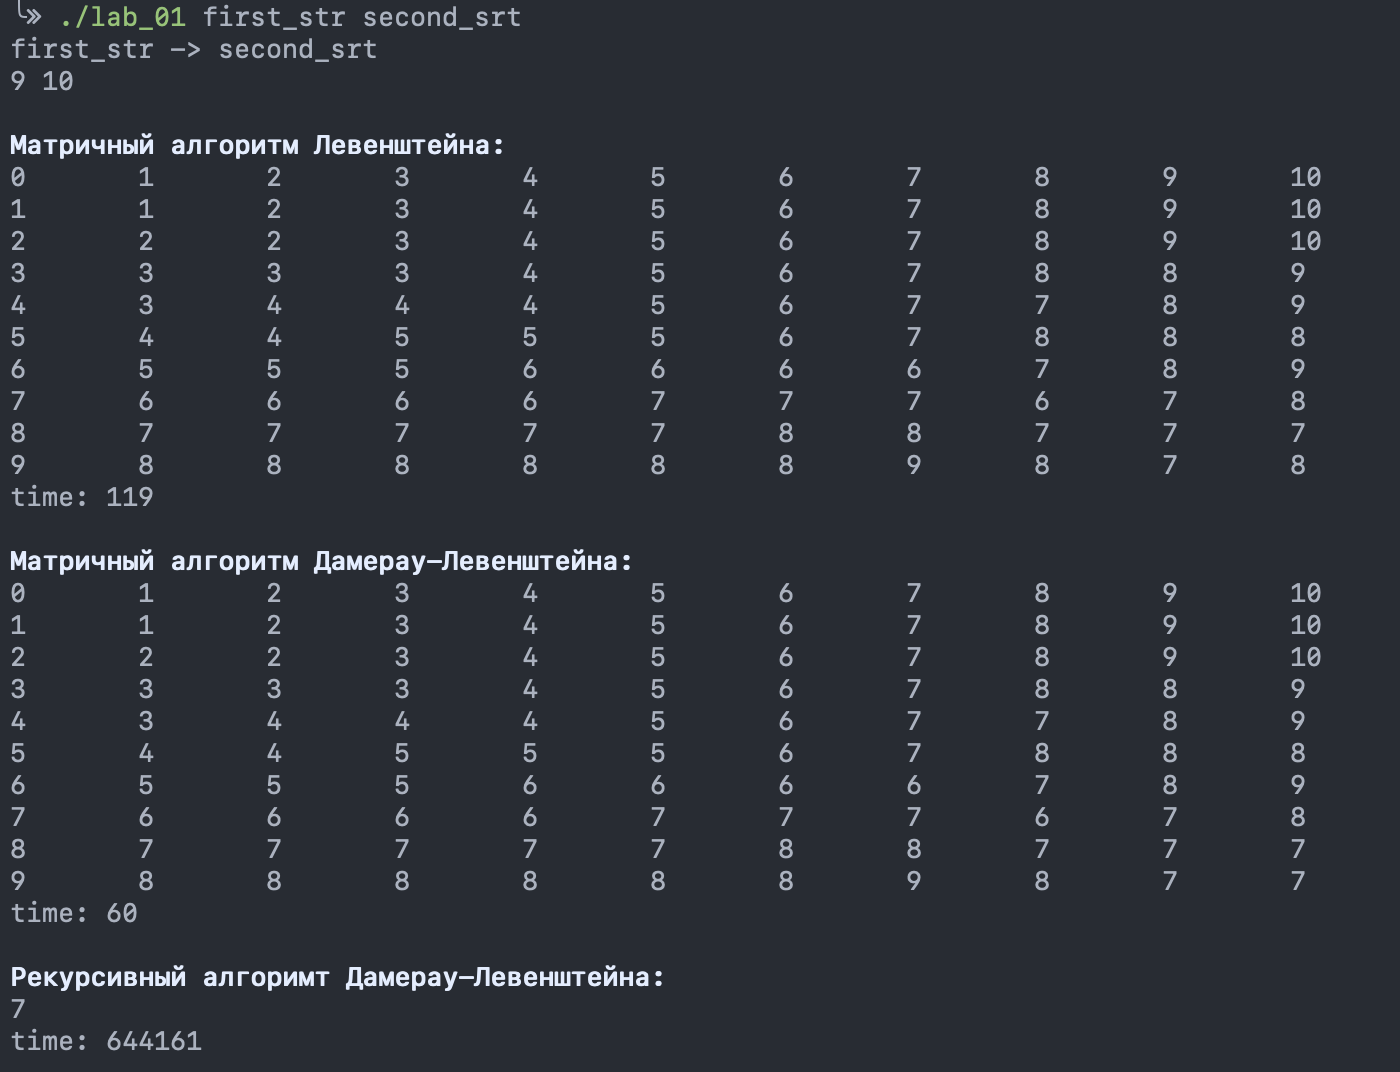
\includegraphics[scale=0.5]{good_work}

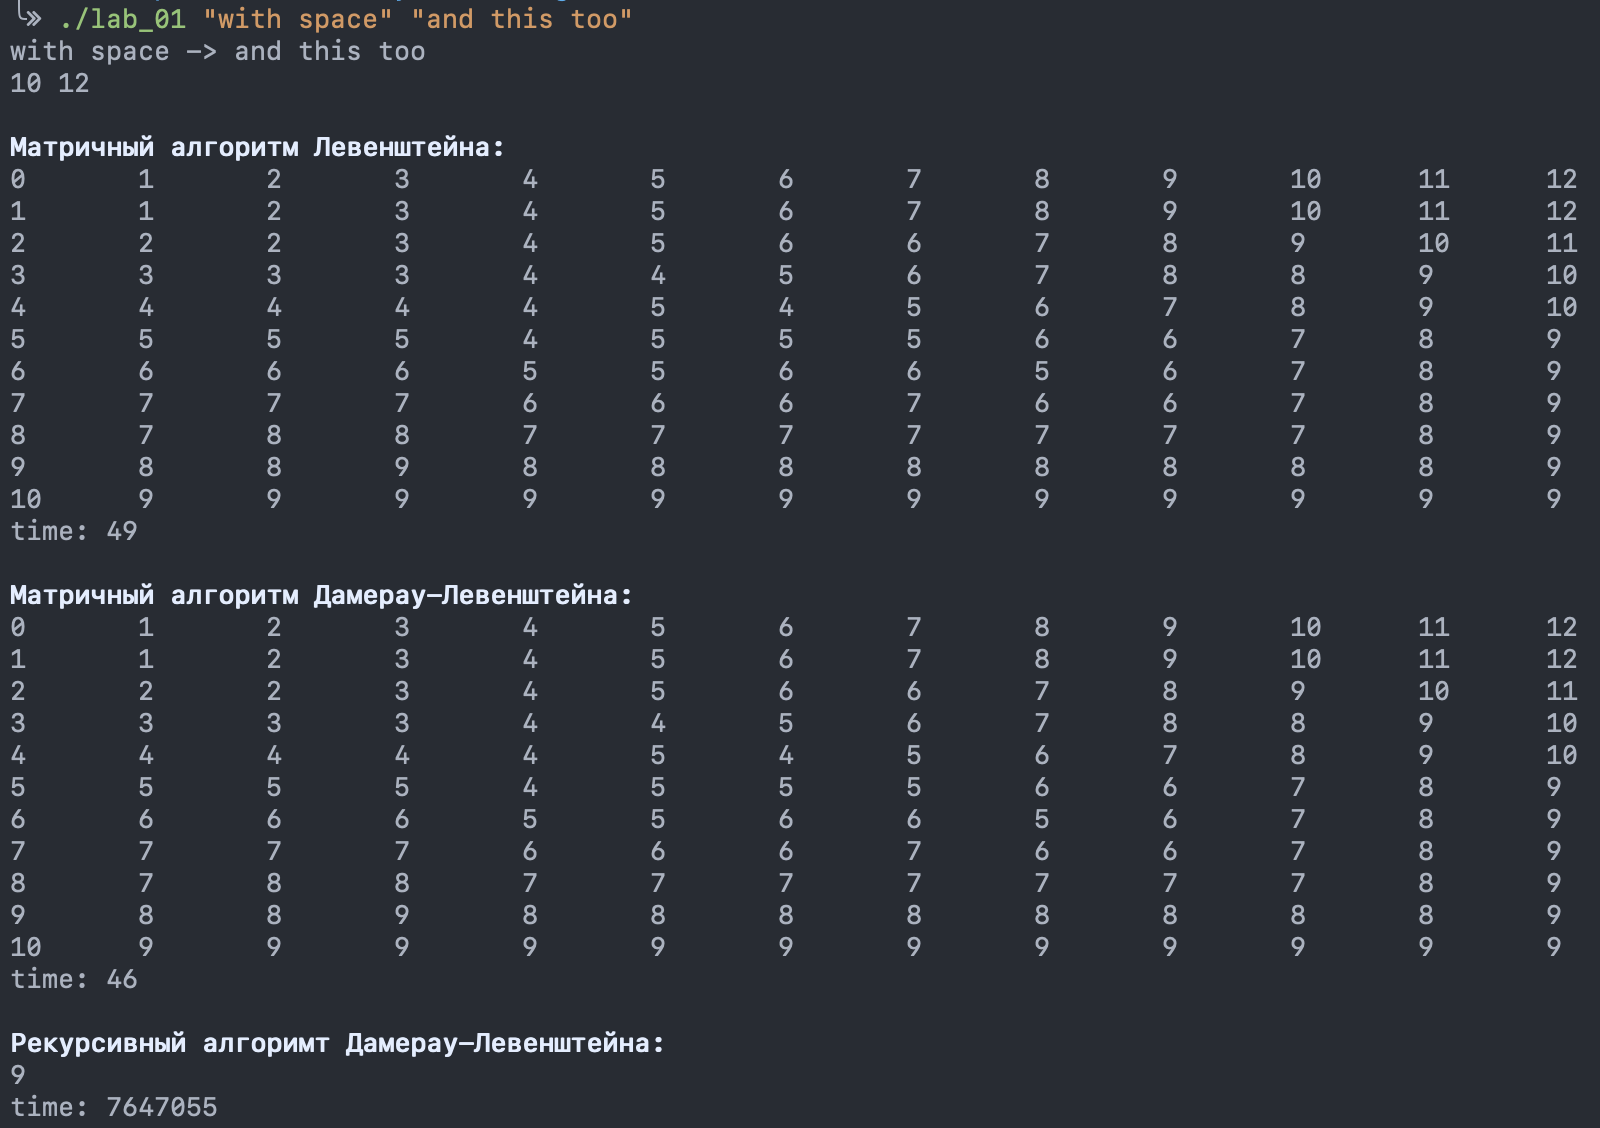
\includegraphics[scale=0.5]{good_space}

\subsection{Результаты тестирования}

Для тестирования были использованы тесты из Таблицы 1 для расстояния
Левенштейна и из Таблицы 2 для расстояния Дамерау-Левенштейна. Ниже
приведены результаты.

\begin{center}
    \begin{tabular}{|c|c|c|}
        \hline
        $s_1$ & $s_2$ & Результат \\
        \hline
        word & word & 0 \\
        \hline
        word & another & 6 \\
        \hline
        ab & ba & 2 \\
        \hline
        qwerty & qwetry & 2 \\
        \hline
        abcdef & badcfe & 4 \\
        \hline
        werylongword & sh & 12 \\
        \hline
        sh & werylongword & 12 \\
        \hline
        wednesday & weekend & 5 \\
        \hline
        memory & mem & 3 \\
        \hline
        feature & erutaef & 6 \\
        \hline
    \end{tabular}

    Таблица 3. Результаты тестирования матричного алгоритма Левенштейна
\end{center}

\hfill

\begin{center}
    \begin{tabular}{|c|c|c|}
        \hline
        $s_1$ & $s_2$ & Результат \\
        \hline
        word & word & 0 \\
        \hline
        word & another & 6 \\
        \hline
        ab & ba & 1 \\
        \hline
        qwerty & qwetry & 1 \\
        \hline
        abcdef & badcfe & 3 \\
        \hline
        werylongword & sh & 12 \\
        \hline
        sh & werylongword & 12 \\
        \hline
        wednesday & weekend & 5 \\
        \hline
        memory & mem & 3 \\
        \hline
        feature & erutaef & 5 \\
        \hline
    \end{tabular}

    Таблица 4. Результаты тестирования матричного алгоритма Дамерау-Левенштейна
\end{center}

\hfill

\begin{center}
    \begin{tabular}{|c|c|c|}
        \hline
        $s_1$ & $s_2$ & Результат \\
        \hline
        word & word & 0 \\
        \hline
        word & another & 6 \\
        \hline
        ab & ba & 1 \\
        \hline
        qwerty & qwetry & 1 \\
        \hline
        abcdef & badcfe & 3 \\
        \hline
        werylongword & sh & 12 \\
        \hline
        sh & werylongword & 12 \\
        \hline
        wednesday & weekend & 5 \\
        \hline
        memory & mem & 3 \\
        \hline
        feature & erutaef & 5 \\
        \hline
    \end{tabular}

    Таблица 5. Результаты тестирования рекурсивного алгоритма Дамерау-Левенштейна
\end{center}

\subsection{Замеры времени}

\begin{tikzpicture}
    \begin{axis}[
        title = Две строки одинаковой длины,
        legend pos = north west,
        xlabel=длина строки,
        ylabel=милисекунды,
        grid = major,
        width = 0.8\paperwidth,
        height = 0.38\paperheight,
        line width = 1
    ]
        \legend{
            Левенштейна матричный,
            Дамерау-Левенштейна матричный
        };
        \addplot[dashed] coordinates {
            (1, 21) (11, 69) (21, 173) (31, 207) (41, 253) (51, 334) (61, 459)
            (71, 586) (81, 733) (91, 894) (101, 1068) (111, 1272) (121, 1582)
            (131, 1793) (141, 1965) (151, 2249) (161, 2519) (171, 2875) (181, 3124)
            (191, 3454) (201, 3824) (211, 4163) (221, 4537) (231, 4947) (241, 5350)
            (251, 5846) (261, 6273) (271, 6714) (281, 7197)(291, 7692) (301, 8200)
            (311, 8732) (321, 9294) (331, 9910) (341, 10423) (351, 11053)
            (361, 11712) (371, 12255) (381, 12946) (391, 14380) (401, 14273)
            (411, 14967) (421, 16551) (431, 16462) (441, 17834) (451, 17905)
            (461, 18692) (471, 19508) (481, 20398) (491, 21116) (501, 21935)
            (511, 22856) (521, 23759) (531, 25452) (541, 25560) (551, 26465)
            (561, 27462) (571, 28427) (581, 29354) (591, 30364) (601, 32142)
            (611, 32342) (621, 33412)(631, 34488) (641, 35643) (651, 37557)
            (661, 37815) (671, 38913) (681, 40069) (691, 41210) (701, 43297)
            (711, 43662) (721, 44888) (731, 46020) (741, 48071) (751, 48514)
            (761, 50870) (771, 51908) (781, 52428) (791, 53698) (801, 56195)
            (811, 56428) (821, 58004) (831, 60044) (841, 60716) (851, 62074)
            (861, 64387) (871, 65186) (881, 66467) (891, 68890) (901, 69687)
            (911, 71000) (921, 73384) (931, 74307) (941, 75929) (951, 78094)
            (961, 78907) (971, 81691) (981, 82229) (991, 84874) (1001, 85432)
        };

        \addplot[black] coordinates {
            (1, 38) (11, 128) (21, 139) (31, 228) (41, 344) (51, 518) (61, 666)
            (71, 854) (81, 1069) (91, 1311) (101, 1579) (111, 1868) (121, 2200)
            (131, 2536) (141, 2916) (151, 3295) (161, 3712) (171, 4155) (181, 4623)
            (191, 5138) (201, 5722) (211, 6186) (221, 6769) (231, 7341) (241, 7931)
            (251, 9433) (261, 9270) (271, 9968) (281, 10683) (291, 11447)
            (301, 12186) (311, 12965) (321, 13799) (331, 14616) (341, 15496)
            (351, 16361) (361, 17295) (371, 18243) (381, 19280) (391, 21172)
            (401, 21229) (411, 22291) (421, 23314) (431, 24364) (441, 25528)
            (451, 26652) (461, 27790) (471, 29738) (481, 30228) (491, 31511)
            (501, 32721) (511, 34028) (521, 35319) (531, 37485) (541, 38017)
            (551, 39406) (561, 40880) (571, 42423) (581, 44504) (591, 45211)
            (601, 46674) (611, 48256) (621, 50721) (631, 51399) (641, 53054)
            (651, 54595) (661, 57060) (671, 57967) (681, 59664) (691, 62451)
            (701, 63143) (711, 66155) (721, 67608) (731, 68549) (741, 71177)
            (751, 72301) (761, 74290) (771, 76833) (781, 77971) (791, 80081)
            (801, 83015) (811, 84006) (821, 86975) (831, 90937) (841, 95018)
            (851, 104317) (861, 101147) (871, 98193) (881, 100037) (891, 103757)
            (901, 103782) (911, 106270) (921, 109067) (931, 111496) (941, 112822)
            (951, 115654) (961, 118642) (971, 120473) (981, 123186) (991, 126838)
            (1001, 127906)
        };
    \end{axis}
\end{tikzpicture}

\begin{tikzpicture}
    \begin{axis}[
        title = Две строки одинаковой длины,
        legend pos = north west,
        xlabel=длина строки,
        ylabel=милисекунды,
        grid = major,
        width = 0.8\paperwidth,
        height = 0.38\paperheight,
        line width = 1
    ]
        \legend{
            Дамерау-Левенштейна матричный,
            Дамерау-Левенштейна рекурсивный
        };
        \addplot[black] coordinates {
            (1, 11) (2, 14) (3, 16) (4, 24) (5, 26) (6, 29) (7, 34) (8, 46) (9, 46)
                        };
        \addplot[dotted] coordinates {
            (1, 3) (2, 10) (3, 22) (4, 183) (5, 338) (6, 2218) (7, 9417) (9, 56574)

        };
    \end{axis}
\end{tikzpicture}

\begin{tikzpicture}
    \begin{axis}[
        title = Одна строка длины 10 вторая - переменной длины,
        legend pos = north west,
        xlabel=длина строки,
        ylabel=милисекунды,
        grid = major,
        width = 0.8\paperwidth,
        height = 0.38\paperheight,
        line width = 1
    ]
        \legend{
            Левенштейна матричный,
            Дамерау-Левенштейна матричный
        };
        \addplot[dashed] coordinates {
            (1, 17) (11, 34) (21, 43) (31, 61) (41, 70) (51, 82) (61, 102)
            (71, 115) (81, 125) (91, 158) (101, 149) (111, 161) (121, 184)
            (131, 196) (141, 209) (151, 220) (161, 239) (171, 244) (181, 259)
            (191, 306) (201, 281) (211, 292) (221, 305) (231, 316) (241, 328)
            (251, 363) (261, 374) (271, 386) (281, 398) (291, 413) (301, 422)
            (311, 435) (321, 448) (331, 459) (341, 471) (351, 484) (361, 498)
            (371, 507) (381, 524) (391, 533) (401, 545) (411, 559) (421, 573)
            (431, 581) (441, 593) (451, 605) (461, 618) (471, 629) (481, 642)
            (491, 654) (501, 666) (511, 721) (521, 733) (531, 745) (541, 759)
            (551, 772) (561, 781) (571, 794) (581, 805) (591, 818) (601, 830)
            (611, 845) (621, 886) (631, 867) (641, 890) (651, 890) (661, 903)
            (671, 915) (681, 926) (691, 939) (701, 954) (711, 963) (721, 975)
            (731, 989) (741, 1000) (751, 1010) (761, 1025) (771, 1036)
            (781, 1127) (791, 1199) (801, 1076) (811, 1085) (821, 1096)
            (831, 1109) (841, 1121) (851, 1156) (861, 1158) (871, 1158)
            (881, 1167) (891, 1182) (901, 1192) (911, 1207) (921, 1217)
            (931, 1229) (941, 1243) (951, 1268) (961, 1267) (971, 1277)
            (981, 1289) (991, 1317) (1001, 1314)
        };

        \addplot[black] coordinates {
            (1, 36) (11, 43) (21, 56) (31, 77) (41, 96) (51, 114) (61, 132)
            (71, 150) (81, 165) (91, 182) (101, 198) (111, 214) (121, 241)
            (131, 259) (141, 275) (151, 291) (161, 308) (171, 325) (181, 341)
            (191, 357) (201, 374) (211, 391) (221, 407) (231, 424) (241, 440)
            (251, 478) (261, 495) (271, 514) (281, 527) (291, 544) (301, 561)
            (311, 577) (321, 595) (331, 612) (341, 627) (351, 644) (361, 660)
            (371, 679) (381, 694) (391, 709) (401, 727) (411, 742) (421, 759)
            (431, 776) (441, 833) (451, 998) (461, 843) (471, 843) (481, 859)
            (491, 876) (501, 892) (511, 953) (521, 969) (531, 984) (541, 1001)
            (551, 1024) (561, 1038) (571, 1055) (581, 1069) (591, 1106)
            (601, 1101) (611, 1115) (621, 1135) (631, 1151) (641, 1168)
            (651, 1187) (661, 1200) (671, 1217) (681, 1234) (691, 1253)
            (701, 1277) (711, 1286) (721, 1301) (731, 1320) (741, 1339)
            (751, 1346) (761, 1364) (771, 1400) (781, 1397) (791, 1415)
            (801, 1430) (811, 1447) (821, 1463) (831, 1480) (841, 1499)
            (851, 1743) (861, 1530) (871, 1549) (881, 1563) (891, 1579)
            (901, 1596) (911, 1611) (921, 1627) (931, 1646) (941, 1664)
            (951, 1678) (961, 1695) (971, 1710) (981, 1727) (991, 1746)
            (1001, 1765)
        };
    \end{axis}
\end{tikzpicture}

\begin{tikzpicture}
    \begin{axis}[
        title = Одна строка длины 10 вторая - переменной длины,
        legend pos = north west,
        xlabel=длина строки,
        ylabel=милисекунды,
        grid = major,
        width = 0.8\paperwidth,
        height = 0.38\paperheight,
        line width = 1
    ]
        \legend{
            Дамерау-Левенштейна матричный,
            Дамерау-Левенштейна рекурсивный
        };
        \addplot[black] coordinates {
            (1, 32) (2, 14) (3, 18) (4, 32) (5, 107) (6, 58) (7, 41) (8, 43) (9, 99)
        };

        \addplot[dotted] coordinates {
            (1, 19) (2, 65) (3, 474) (4, 2537) (5, 11512) (6, 36962) (7, 107236) (8, 355532) (9, 902894)
        };
    \end{axis}
\end{tikzpicture}

\subsection{Выводы}

Из графиков отношения времени к длинам строк видно, что рекурсивный
алгоритм сильно проигрывает матричным. Поэтому выгонее использовать
матричные алгоритмы. Также видно, что алгоритм Дамерау-Левенштейна на 25\%
проигрывает обычному алгоритму Левенштейна на строках длины больше 400.

\newpage
\anonsection{Заключение}

В ходе данной работы было выполнено сравнение трех алгоритмов нахождения минимального редакционного расстояния для двух строк: расстояния Левенштейна матричным методом, расстояния Дамерау-Левенштейна матричным и рекурсивным методами. Данные алгоритмы широко используются для поисковиков, в которых необходимо выявлять оошибки при наборе текста, для сравнения белков и генов в биоинформатике, а также для утилит diff.

Было проведено сравнение времени всех алгоритмов для случая, когда две строки имееют одинаковую длину и для случая, когда одна строка небольшая, а вторая варьрируется. В ходе этого исследования были сделаны следующие выводы:

\begin{enumerate}
    \item[1)] рекурсивная реализация сильно проигрывает матричной реализации, и ее невыгодно использовать ни в одном случае;
    \item[2)] матричный алгоритм нахождения расстояния Дамерау-Левенштейна работает на 25\% медленнее, чем Левенштейна за счет рассчета дополнительного действия смены соседних букв, что дает более хороший результат.
\end{enumerate}

\newpage
% даём указание на включение данного место в оглавление как секции (\section)
\addcontentsline{toc}{section}{Список используемой литературы}

%далее сам список используевой литературы
\begin{thebibliography}{}
    \bibitem{binlev} Владимир И. Левенштейн - "Двоичные коды с исправлением выпадений, вставок и замещений символов"
    \bibitem{habr} Нечёткий поиск в тексте и словаре - https://habr.com/ru/post/114997/ [Электронный ресурс] Дата орбращения: 04.10.2019
    \bibitem{bio} Гасфилд - "Строки, деревья и последовательности в алгоритмах. Информатика и вычислительная биология. Невский Диалект БВХ-Петербург, 2003.
    \bibitem{itmo} Задача о редакционном расстоянии - 

    https://neerc.ifmo.ru/wiki/index.php?title=Задача\_о\_редакционном\_расстоянии,\_алгоритм\_Вагнера-Фишера [Электронный ресурс] Дата обращения: 04.10.2019

    \bibitem{bmstu} Желудков А. В., Макаров Д. В., Фадеев П. В. - "Особенности алгоритмов нечёткого поиска" Инженерный вестник 2014
\end{thebibliography}

\end{document}
